\documentclass{report}

\usepackage[utf8]{inputenc}
\usepackage[T1, T2A]{fontenc}
\usepackage[english, russian]{babel}
\usepackage{csquotes}

\usepackage{array}


\usepackage[
    backend = biber,
    style = numeric,
]{biblatex}

\addbibresource{Refs.bib}


\usepackage{graphicx}
\graphicspath{ {./images/} }


\title{Моделирование частотных сканов}
\author{Богачев А.М.}
\date{\today}


\begin{document}
    \maketitle


    \chapter{Цели и задачи}

    Согласно источнику \cite{istratov_exp_analysis} Сигналы релаксации ёмкости 
    барьерных структур можно условно разделить на три группы:
    \begin{enumerate}
        \item Моноэкспоненциальный сигнал релаксации, обусловленный одним единственным 
        энергетическим уровнем в запрещённой зоне полупроводника.
        \item Сигнал релаксации, состоящий из суммы нескольких моноэкспоненциальных 
        сигналов релаксации.
        \item Сигнал релаксации, характеризуемый непрерывным распределением скоростей 
        эмиссии, представленным спектральной функцией $g(\lambda)$.
    \end{enumerate}

    Таким образом, цель работы по моделированию частотных сканов в самом общем виде 
    можно описать следующим образом: найти способ определять спектральную функцию 
    $g(\lambda)$, её параметры, а также зависимость этих параметров от температуры.

    Для достижения поставленной цели нужно решить предположительно следующие задачи:
    \begin{enumerate}
        \item Разработать алгоритм идентификации частотного скана 
        моноэкспоненциального сигнала релаксации.
        \item Разработать алгоритм идентификации частотного скана 
        неэкспоненциального сигнала релаксации с показателем $p$, 
        характеризующим нелинейность и неэкспоненциальность.
        \item Разработать программу идентификации частотного 
        скана сигнала релаксации, состоящего из суммы моноэкспоненциальных 
        сигналов. Программа должна определять параметры каждого 
        моноэкспоненциального сигнала.
        \item Разработать программу идентификации группы частотных сканов 
        при разных температурах. На данном этапе предполагается, что сигнал 
        релаксации образован суммой моноэкспоненциальных сигналов, 
        количество которых не меняется в зависимости от температуры, 
        меняются только их параметры.
        \item Разработать программу иденитификации спектральной 
        функции $g(\lambda)$ и её параметров для отдельного 
        частотного скана.
        \item Разработать программу иденитификации спектральной 
        функции $g(\lambda)$ и её параметров для группы частотных сканов при 
        разных температурах, полагая, что от температуры зависят только 
        параметры $g(\lambda)$.
    \end{enumerate}


    \chapter{Моделирование частотных сканов с одной экспоненциальной 
    составляющей без показателя $p$}

    \section{Подготовка данных}
        Выходной сигнал коррелятора спектрометра DLS-82E определяется 
        выражением \ref{eq:eq1}.

        \begin{equation}
            \label{eq:eq1}
            S\left(\tau,C_A,F_0, t_1\right) = C_A K_{BS} K_{LS} \phi\left(\tau,F_0,t_1\right),
        \end{equation}
        где
        \begin{description}
            \item[$C_A$] -- амплитуда емкостного релаксационного сигнала,
            \item[$K_{BS}$] -- масштабный коэффициент, зависящий от чувствительности 
            емкостного моста,
            \item[$K_{LS}$] -- масштабный коэффициент селектора,
            \item[$\tau$] -- постоянная времени релаксации гулбокого уровня,
            \item[$F_0$] -- частота сканирования импульсов заполнения,
            \item[$t_1$] -- длительность импульса заполнения,
            \item[$\phi\left(\tau,F_0,t_1\right)$] -- функция определяемая выражением
            \ref{eq:eq2}.
        \end{description}
        \begin{equation}
            \label{eq:eq2}
            \phi\left(\tau,F_0,t_1\right) = 
            M \tau F_0 e^{-\frac{0.05}{\tau F_0}}
            \left(1-e^{\frac{t_1 F_0-0.45}{\tau F_0}}
            -e^{-\frac{0.5}{\tau F_0}}+
            e^{\frac{t_1 F_0-0.95}{\tau F_0}}\right),
        \end{equation}
        где $M$ -- масштабный множитель.

        Введём коэффициент A, характеризующий амплитуду сигнала релаксации ёмкости:
        \begin{equation}
            \label{eq:eq3}
            A=C_A K_{BS} K_{LS}.
        \end{equation}

        При моделировании будем считать масштабный коэффициент и длительность импульса 
        заполнения постоянными: \(t_1 = 20 \cdot 10^{-6} c\), \(M = 5.861\).

        При идентификации параметров модели будем определять коэффициент $A$, 
        характеризующий амплитуду сигнала релаксации, и постоянную времени сигнала 
        релаксации $\tau$.

        Так как выражения \ref{eq:eq1} и \ref{eq:eq2} при моделировании будут зависеть 
        только от трёх параметров: $\tau$, $A$, $F_0$, их левые части можно переписать 
        следующим образом:
        \begin{equation}
            \label{eq:eq4}
            S\left(\tau,A,F_0\right) = A \phi\left(\tau,F_0\right),
        \end{equation}
        \begin{equation}
            \label{eq:eq5}
            \phi\left(\tau,F_0\right) = 
            M \tau F_0 e^{-\frac{0.05}{\tau F_0}}
            \left(1-e^{\frac{t_1 F_0-0.45}{\tau F_0}}
            -e^{-\frac{0.5}{\tau F_0}}+
            e^{\frac{t_1 F_0-0.95}{\tau F_0}}\right).
        \end{equation}

        Подготовим исходные данные для моделирования. На первом этапе предлагается 
        использовать расчётные данные вместо экспериментальных, чтобы можно было 
        оценить качество идентификации параметров модели. 

        Подготовим массив значений частоты, распределённых равномерно по логарифму 
        частоты. Каждое значение вычисляется по следующей формуле \ref{eq:eq6}.
        \begin{equation}
            \label{eq:eq6}
            F_{0_i} = 10 ^ {\left(i-1\right)d},
        \end{equation}
        \begin{description}
            \item[$i$] -- номер элемента в массиве (от $1$ до $N$; $N$ – количество 
            элементов в массиве),
            \item[$d$] -- шаг по логарифму частоты, который вычисляется 
            автоматически в программе моделирования.
        \end{description}

        В таблице \ref{table:table1} приведены параметры массива частот.

        \begin{table}[ht]
            \label{table:table1}
            \caption{Параметры массива частот}
            \centering
            \begin{tabular}{ | m{2.0cm} | m{2.0cm} | m{2.5cm} | m{2.5cm} | }
                \hline
                Параметр & Начальная частота, Гц & Конечная частота, Гц & Количество значений \\
                \hline
                Значения & 1 & 2500 & 1000 \\
                \hline
            \end{tabular}
        \end{table}

        Для каждого значения частоты вычислим значения выходного сигнала 
        коррелятора по формуле \ref{eq:eq7}.
        \begin{equation}
            \label{eq:eq7}
            S^*\left(\tau,A,F_0\right) = A\phi\left(\tau,F_0\right) + n(\mu, \sigma),
        \end{equation}
        где $n$ -- нормально распределённый шум с математическим ожиданием 
        $\mu$ и среднеквадратическим отклонением $\sigma$.
        
        Для расчётов будем использовать параметры, перечисленные в таблице~\ref{table:table2}.

        \begin{table}[ht]
            \caption{Параметры для вычисления исходных данных}
            \label{table:table2}
            \centering
            \begin{tabular}{ | l | c | c | c | c | }
                \hline
                Параметр & $\tau$,c & $A$ & $\mu$ & $\sigma$ \\
                \hline
                Значение & 0.005 & 3.0 & 0 & 0.2 \\
                \hline
            \end{tabular}
        \end{table}

        На рисунке \ref{pic:pic1} показан рассчитанный частотный скан.

        \begin{figure}[ht]
            \centering
            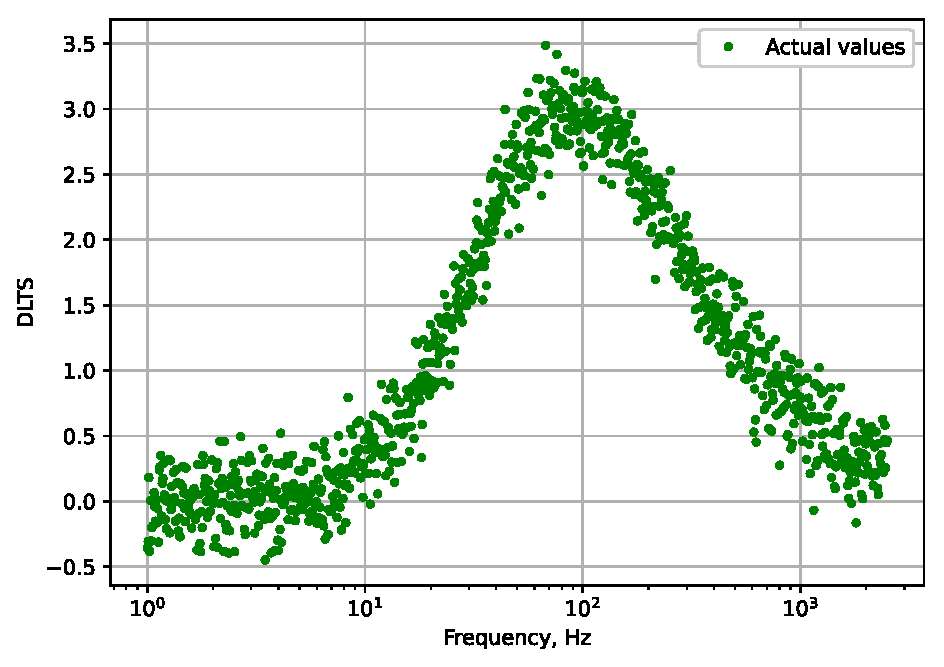
\includegraphics[width=0.75\textwidth]{experimental_data}

            \caption{Рассчитанный частотный скан. По горизонтали 
            отложена частота в Гц, по вертикали -- сигнал DLTS.}
            \label{pic:pic1}
        \end{figure}


        \section{Идентификация параметров модели}
        Идентификацию параметров модели будем проводить нелинейным методом 
        наименьших квадратов.
        
        В качестве целевой функции при оптимизации параметров модели выберем 
        минимум среднеквадратической ошибки между исходными данными и данными, 
        вычисляемыми моделью (формула \ref{eq:eq8}).

        \begin{equation}
            \label{eq:eq8}
            E = \frac{1}{N}\sum_{i=1}^{N}\left(S_i^*-S_i\right)^2
        \end{equation}

        Оптимизацию параметров модели будем выполнять методом стохастического 
        градиентного спуска по мини-батчам (выборкам), так как данный алгоритм 
        обладает высокой скоростью и меньше подвержен риску остановиться 
        в локальном минимуме целевой функции. Размер выборки (параметр 
        \texttt{batch\_size}) зададим равны \texttt{100}, количество итераций 
        (параметр \texttt{epochs} -- <<эпохи>>) также зададим равным \texttt{100}, 
        скорость градиентного спуска (параметр \texttt{learning\_rate}) зададим 
        равным \texttt{0.1}. Данный алгоритм работает следующим образом:
        \begin{enumerate}
            \item из всех исходных данных 100 точек (параметр 
            \texttt{batch\_size}) выбираются случайным образом;
            \item по выбранным точкам выполняется градиентный спуск;
            \item пункты 1 и 2 повторяются \(N/batch\_size\) раз 
            (\(N\) -- количество точек в массиве исходных данных), при 
            каждом повторении фиксируются лучшие параметры модели;
            \item пункты 1 -- 3 повторяются заданное количество раз 
            (параметр \texttt{epochs}), в конце каждой итерации фиксируются 
            лучшие значения параметров.
        \end{enumerate}

        Стохастический градиентный спуск находит решение быстрее и работает стабильнее, 
        если значения параметров модели находятся примерно в одном и том же масштабе. 
        Чтобы выполнить данное условие, будем оптимизировать не постоянную времени 
        $\tau$, а её логарифм, т.е. в выражениях \ref{eq:eq4} и \ref{eq:eq5} заменим 
        $\tau$ выражением \ref{eq:eq9} и будем искать оптимальное значение степени 
        $\rho$ вместо $\tau$.
        \begin{equation}
            \label{eq:eq9}
            \tau = 10^\rho
        \end{equation}

        Данная замена также исключит возможность появления отрицательных значений 
        $\tau$ в результате работы алгоритма оптимизации.

        Начальные значения параметров будем выбирать случайными из диапазонов, 
        приведённых в таблице~\ref{table:table3}.

        \begin{table}[ht]
            \caption{Диапазоны начальных значений параметров}
            \label{table:table3}
            \centering
            \begin{tabular}{ | l | l | l | }
                \hline
                Параметр & Минимальное значение & Максимальное значение \\
                \hline
                $\rho$ & -3 & -0.5 \\
                \hline
                $A$ & 0.3 & 3.3 \\
                \hline
            \end{tabular}
        \end{table}
        
        Не исключено, что вместо произвольных значений правильнее выбирать 
        значения параметров в произвольной точке частотного скана.
        
        На рисунке \ref{pic:pic2} показан результат работы алгоритма идентификации.
        На графике слева показаны исходные данные (зелёные точки), частотный скан, 
        полученный на модели до оптимизации параметров (синяя линия), частотный 
        скан, полученный на модели после оптимизации параметров (красная линия); 
        по горизонтали отложена частота в Гц, по вертикали -- сигнал DLTS. 
        На графике справа показана зависимость среднеквадратической ошибки от 
        количества <<эпох>>.

        \begin{figure}[ht]
            \centering
            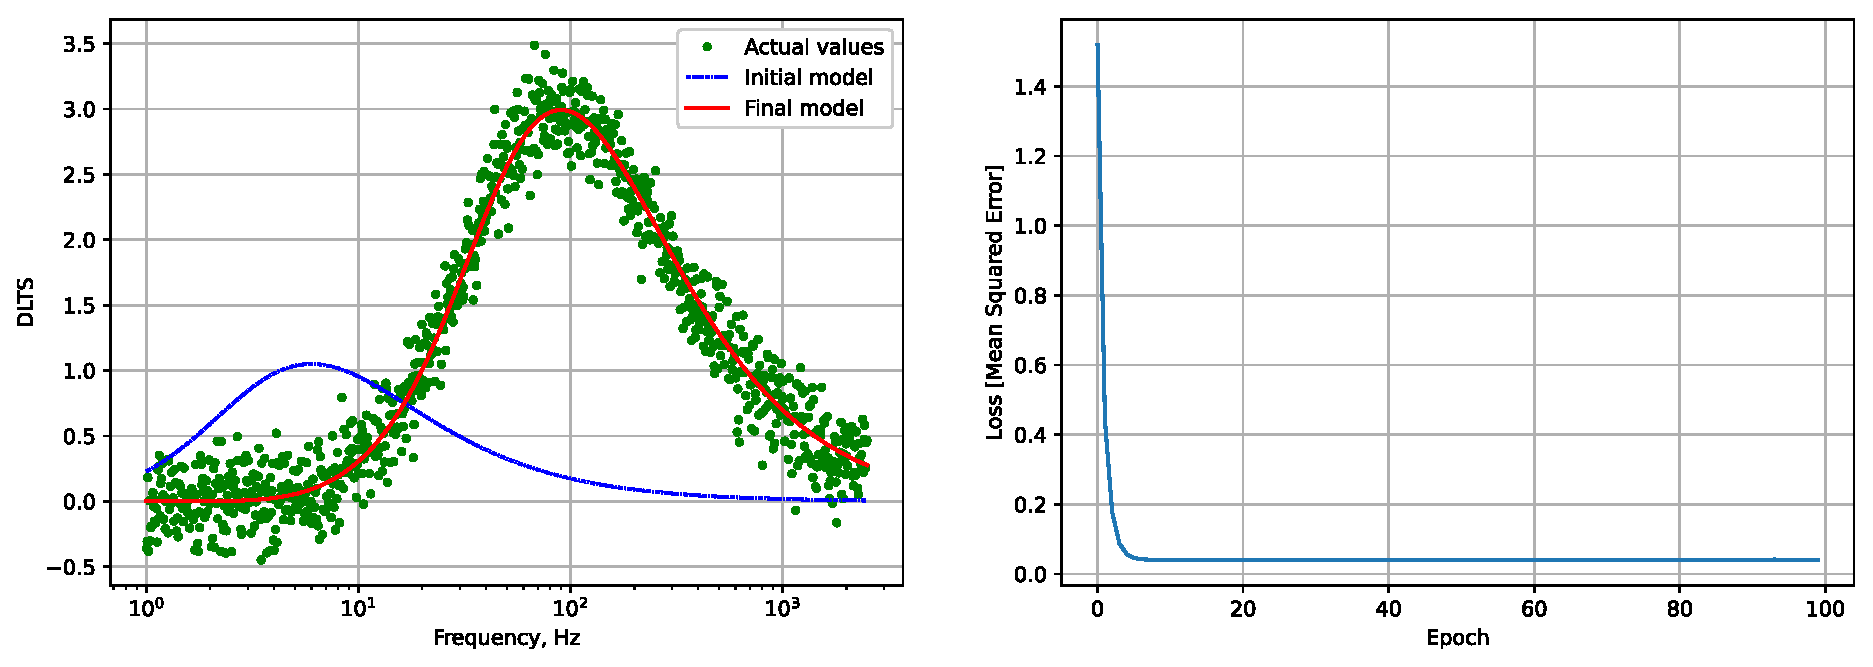
\includegraphics[width=\textwidth]{SGD}
            \caption{Результаты идентификации модели}
            \label{pic:pic2}
        \end{figure}

        В таблице \ref{table:table4} приведены численные значения результатов 
        идентификации модели.
        
        \begin{table}[ht]
            \caption{Результаты идентификации параметров модели}
            \label{table:table4}
            \centering
            \begin{tabular}{ | m{2.5cm} | m{2.5cm} | m{2.5cm} | m{2.5cm} | }
                \hline
                Параметр & Значения до оптимизации & Значения после оптимизации & Исходные значения \\
                \hline
                $A$ & 1.0500 & 2.9973 & 3.0 \\
                \hline
                $\rho$ & -1.133 & -2.312 & --- \\
                \hline
                $\tau$ & 0.0736 & 0.0049 & 0.005 \\
                \hline
                $E$ & 2.1472 & 0.0406 & --- \\
                \hline
                $\sqrt{E}$ & 1.465317 & 0.201380 & ---\\
                \hline
            \end{tabular}
        \end{table}

        Алгоритм достигает сходимости очень быстро, таким образом, нет необходимости 
        использовать вариации градиентного спуска с адаптивной скоростью.


        \chapter{Моделирование частотных сканов с учётом показателя $p$}

        \section{Подготовка данных}
        Для комплексного учёта нелинейности аналогового тракта спектрометра и 
        неэкспоненциальности релаксационного сигнала используется показатель $p$, 
        введя его в выражение \ref{eq:eq4}, получим выражение \ref{eq:eq10}.
        \begin{equation}
            \label{eq:eq10}
            S\left(\tau, A, F_0\right) = A\left[\phi\left(\tau,F_0\right)\right]^p
        \end{equation}

        Рассчитаем экспериментальные данные аналогично тому как это делалось в 
        предыдущей части, но принимая во внимание коэффициент $p$. Для расчёта 
        используется та же сетка частот, что и в предыдущем разделе. Параметры, 
        использованные для расчёта приведены в таблице \ref{table:table5}.

        \begin{table}[ht]
            \caption{Параметры для вычисления исходных данных}
            \label{table:table5}
            \centering
            \begin{tabular}{ | l | c | c | c | c | c |}
                \hline
                Параметр & $\tau$, с & $A$ & $p$ & $\mu$ & $\sigma$ \\
                \hline
                Значение & 0.005 & 3.0 & 1.5 & 0 & 0.2 \\
                \hline
            \end{tabular}
        \end{table}

        На рисунке \ref{pic:pic3} приведён рассчитанный частотный скан.

        \begin{figure}[ht]
            \centering
            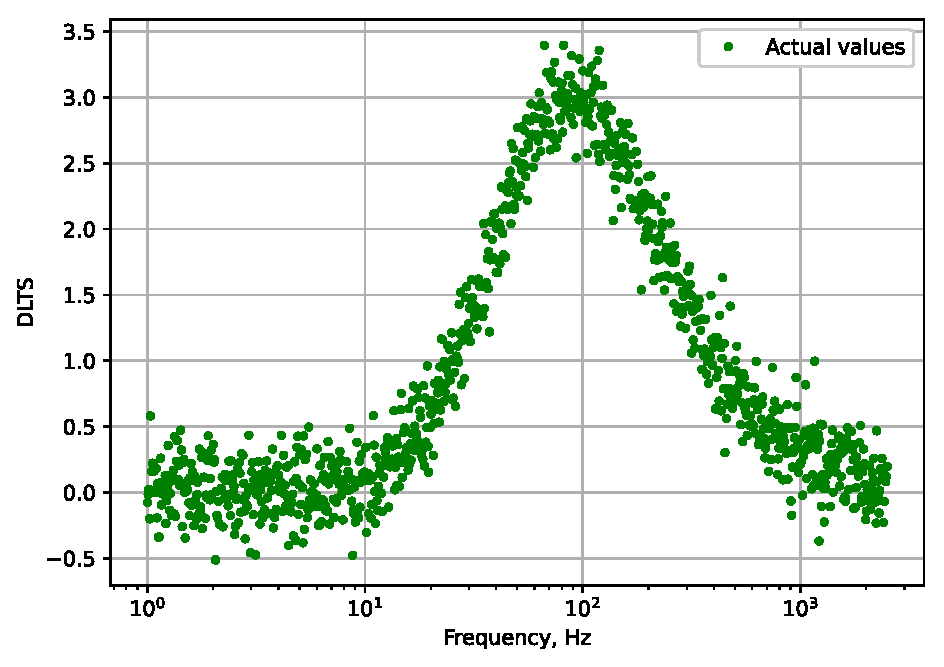
\includegraphics[width=0.75\textwidth]{p_experimental_data}
            \caption{Рассчитанный частотный скан. По горизонтали отложена 
            частота в Гц, по вертикали -- сигнал DLTS.}
            \label{pic:pic3}
        \end{figure}

        \section{Идентификация параметров модели}
        Выполним идентификацию параметров модели тем же способом, что и 
        в предыдущем разделе. Алгоритм и его параметры оставим без изменений, 
        за исключением того, что идентификация теперь проводится по трём 
        параметрам, а параметр $p$ в начале идентификации всегда будет равным $1$.

        На рисунке \ref{pic:pic4} приведён результат работы алгоритма идентификации.
        На графике слева показаны исходные данные (зелёные точки), частотный скан, 
        полученный на модели до оптимизации параметров (синяя линия), частотный скан, 
        полученный на модели после оптимизации параметров (красная линия); по 
        горизонтали отложена частота в Гц, по вертикали – сигнал DLTS. На графике 
        справа показана зависимость среднеквадратической ошибки от количества <<эпох>>.

        \begin{figure}[ht]
            \centering
            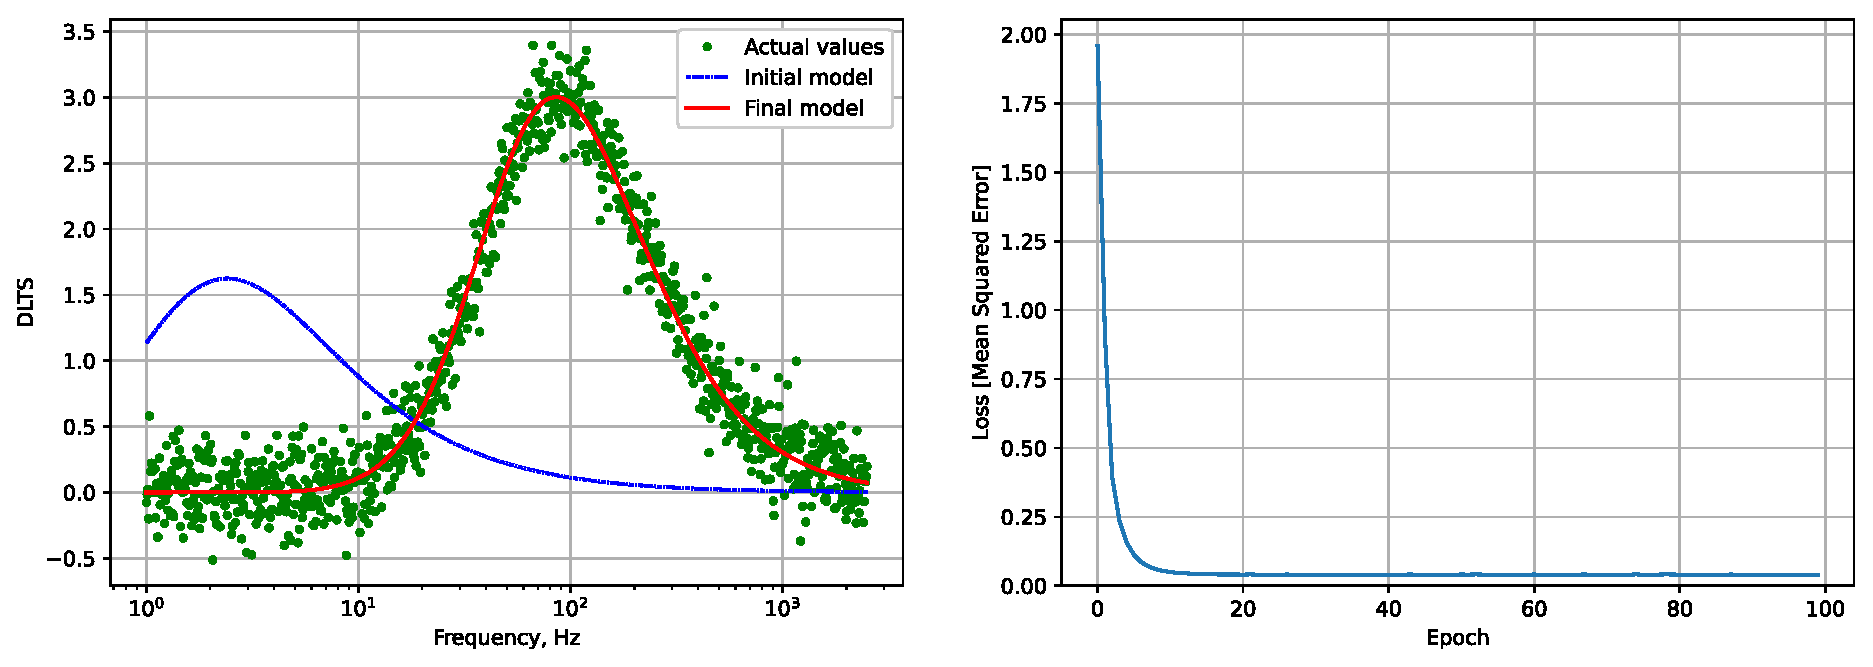
\includegraphics[width=\textwidth]{p_SGD}
            \caption{Результаты идентификации модели}
            \label{pic:pic4}
        \end{figure}

        В таблице \ref{table:table6} приведены численные значения результатов 
        идентификации модели.

        \begin{table}[ht]
            \caption{Результаты идентификации параметров модели.}
            \label{table:table6}
            \centering
            \begin{tabular}{ | m{2.5cm} | m{2.5cm} | m{2.5cm} | m{2.5cm} | }
                \hline
                Параметр & Значения до оптимизации & Значения после оптимизации & Исходные значения \\
                \hline
                $A$ & 1.6234 & 3.0084 & 3.0\\
                \hline
                $\rho$ & -0.7361 & -2.2892 & --- \\
                \hline
                $\tau$ & 0.1836 & 0.0051 & 0.005 \\
                \hline
                $p$ & 1.0 & 1.5225 & 1.5 \\
                \hline
                $E$ & 2.2571 & 0.0404 & --- \\
                \hline
                $\sqrt{E}$ & 1.5024 & 0.2010 & ---\\
                \hline
            \end{tabular}
        \end{table}


        \chapter{Моделирование частотных сканов с несколькими экспоненциальными составляющими}

        \section{Подготовка данных}
        







    
    \printbibliography

\end{document}